\subsection{Authentication Module}
\label{sec:mobile-authentication}

\textbf{Purpose:}
Provides a secure authentication system that allows users to create new accounts, log into the application, and recover forgotten passwords. The authentication module communicates with the backend through REST APIs and securely stores authentication tokens for future requests.

\vspace{0.2cm}
\noindent\textbf{Main Features}

\begin{itemize}
    \item User Login
    \item User Registration
    \item Password Recovery
    \item Form Validation
    \item JWT-based Authentication
\end{itemize}

%%%%%%%%%%%%%%%%%%%%%%%%%%%%%%%%%%%%%%%%%%%%%%%%%%%%%%%%%%%%

\subsubsection{Login Screen}

\textbf{Purpose:}
Allows registered users to securely authenticate using their email address and password before accessing the application.

\begin{figure}[H]
    \centering
    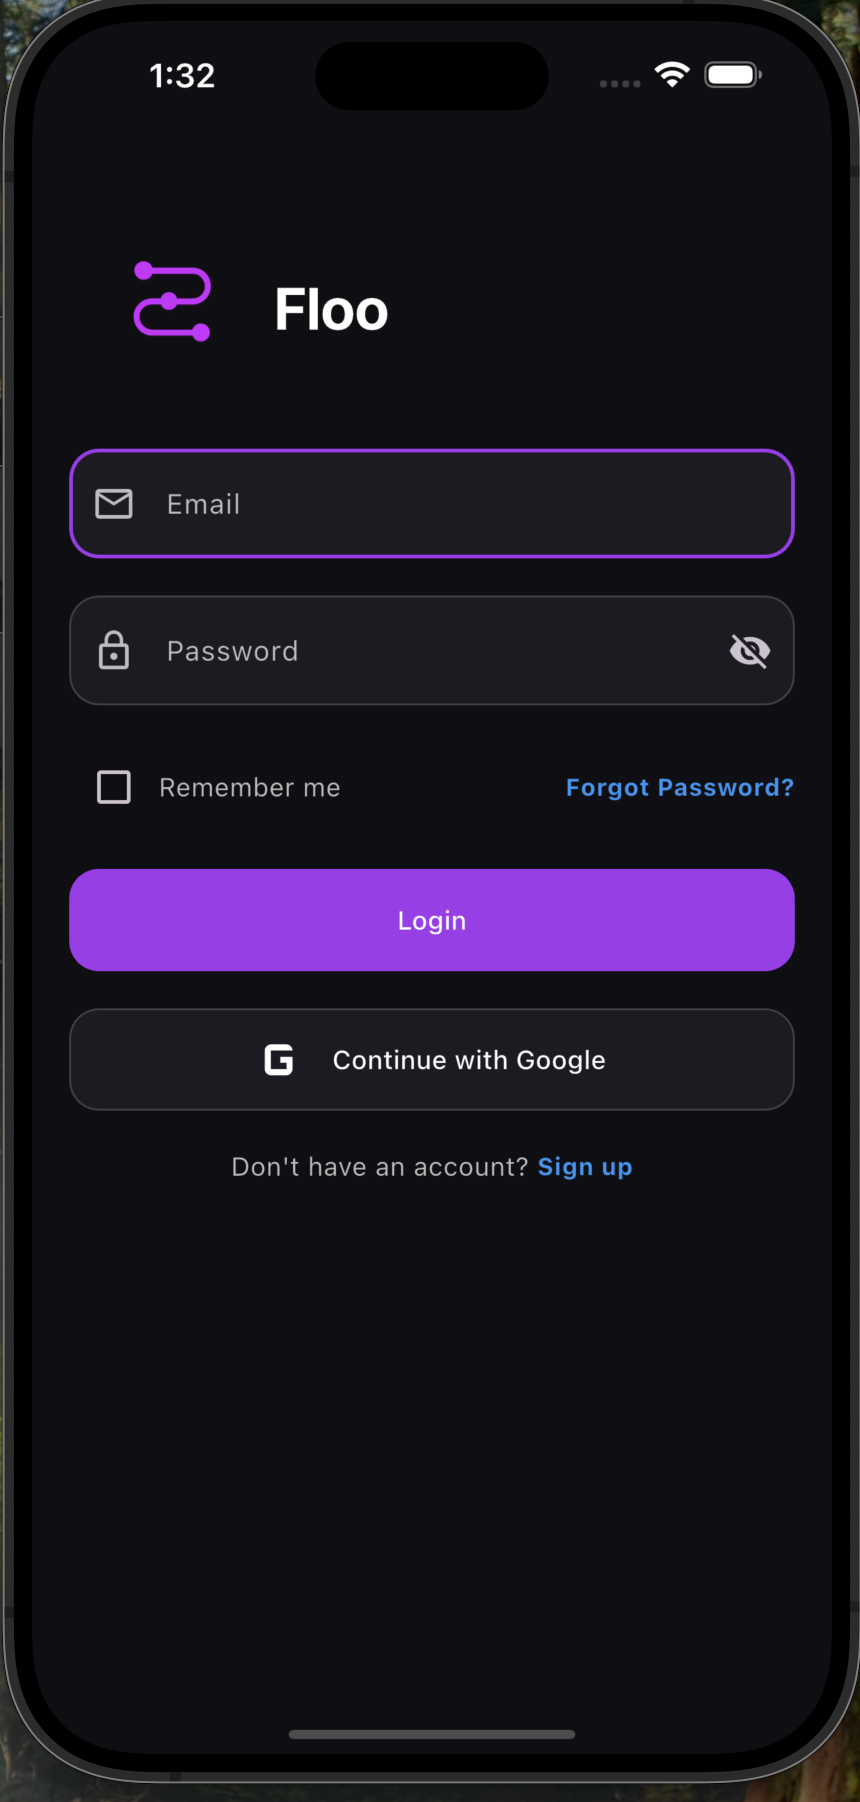
\includegraphics[width=0.42\textwidth]{images/mobile-app/auth-pages/auth-login-D.png}
    \caption{Login Screen}
    \label{fig:mobile-login}
\end{figure}

\vspace{0.2cm}
\noindent\textbf{Main Components}

\begin{itemize}
    \item Email Text Field
    \item Password Text Field
    \item Password Visibility Toggle
    \item Login Button
    \item Forgot Password Button
    \item Navigate to Registration Screen
\end{itemize}

\vspace{0.2cm}
\noindent\textbf{Behavior \& Logical Flows}

\begin{itemize}
    \item Validates email and password fields before sending authentication requests.
    \item Sends login requests to the backend using the Dio HTTP client.
    \item Stores the received JWT access token securely using SharedPreferences.
    \item Redirects authenticated users to the Home screen.
    \item Displays loading indicators during authentication.
    \item Shows descriptive error messages when login fails.
\end{itemize}

%%%%%%%%%%%%%%%%%%%%%%%%%%%%%%%%%%%%%%%%%%%%%%%%%%%%%%%%%%%%

\subsubsection{Registration Screen}

\textbf{Purpose:}
Allows new users to create an account by providing their personal information and login credentials.

\begin{figure}[H]
    \centering
    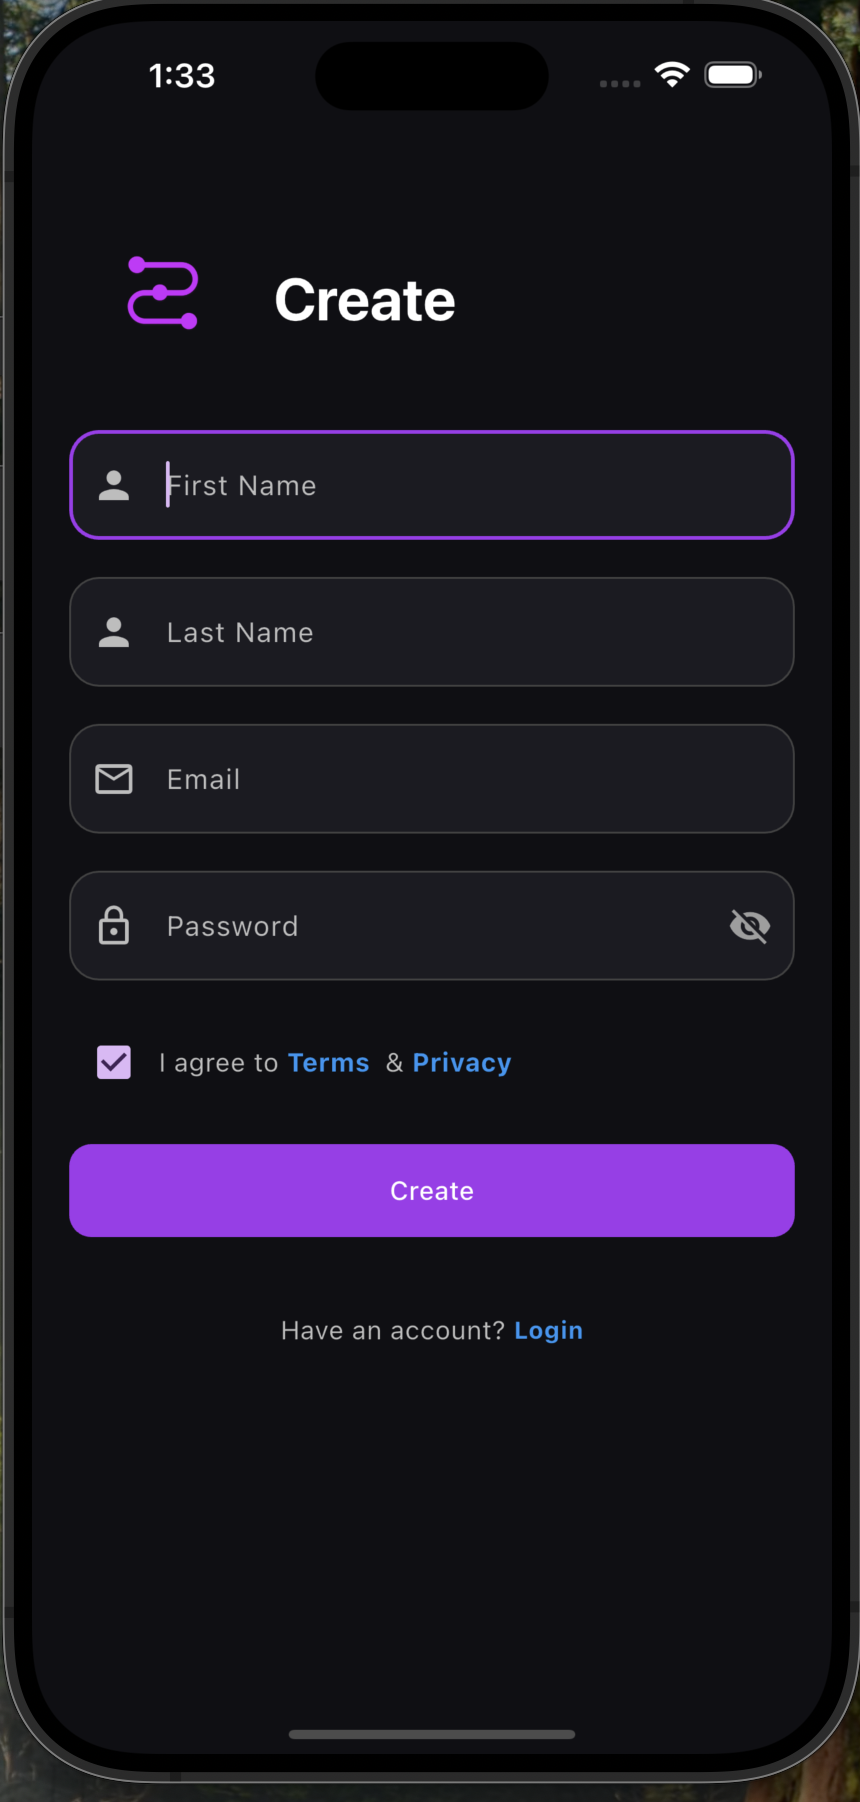
\includegraphics[width=0.42\textwidth]{images/mobile-app/auth-pages/auth-regis_D.png}
    \caption{Registration Screen}
    \label{fig:mobile-register}
\end{figure}

\vspace{0.2cm}
\noindent\textbf{Main Components}

\begin{itemize}
    \item First Name Field
    \item Last Name Field
    \item Email Field
    \item Password Field
    \item Confirm Password Field
    \item Register Button
\end{itemize}

\vspace{0.2cm}
\noindent\textbf{Behavior \& Logical Flows}

\begin{itemize}
    \item Validates all required fields before submitting the registration request.
    \item Ensures that both password fields contain matching values.
    \item Sends registration data securely to the backend.
    \item Displays validation messages whenever invalid data is entered.
    \item Redirects users to the Login screen after successful registration.
\end{itemize}

%%%%%%%%%%%%%%%%%%%%%%%%%%%%%%%%%%%%%%%%%%%%%%%%%%%%%%%%%%%%

\subsubsection{Password Recovery}

\textbf{Purpose:}
Allows users to reset forgotten passwords securely through backend verification.

\begin{figure}[H]
    \centering
    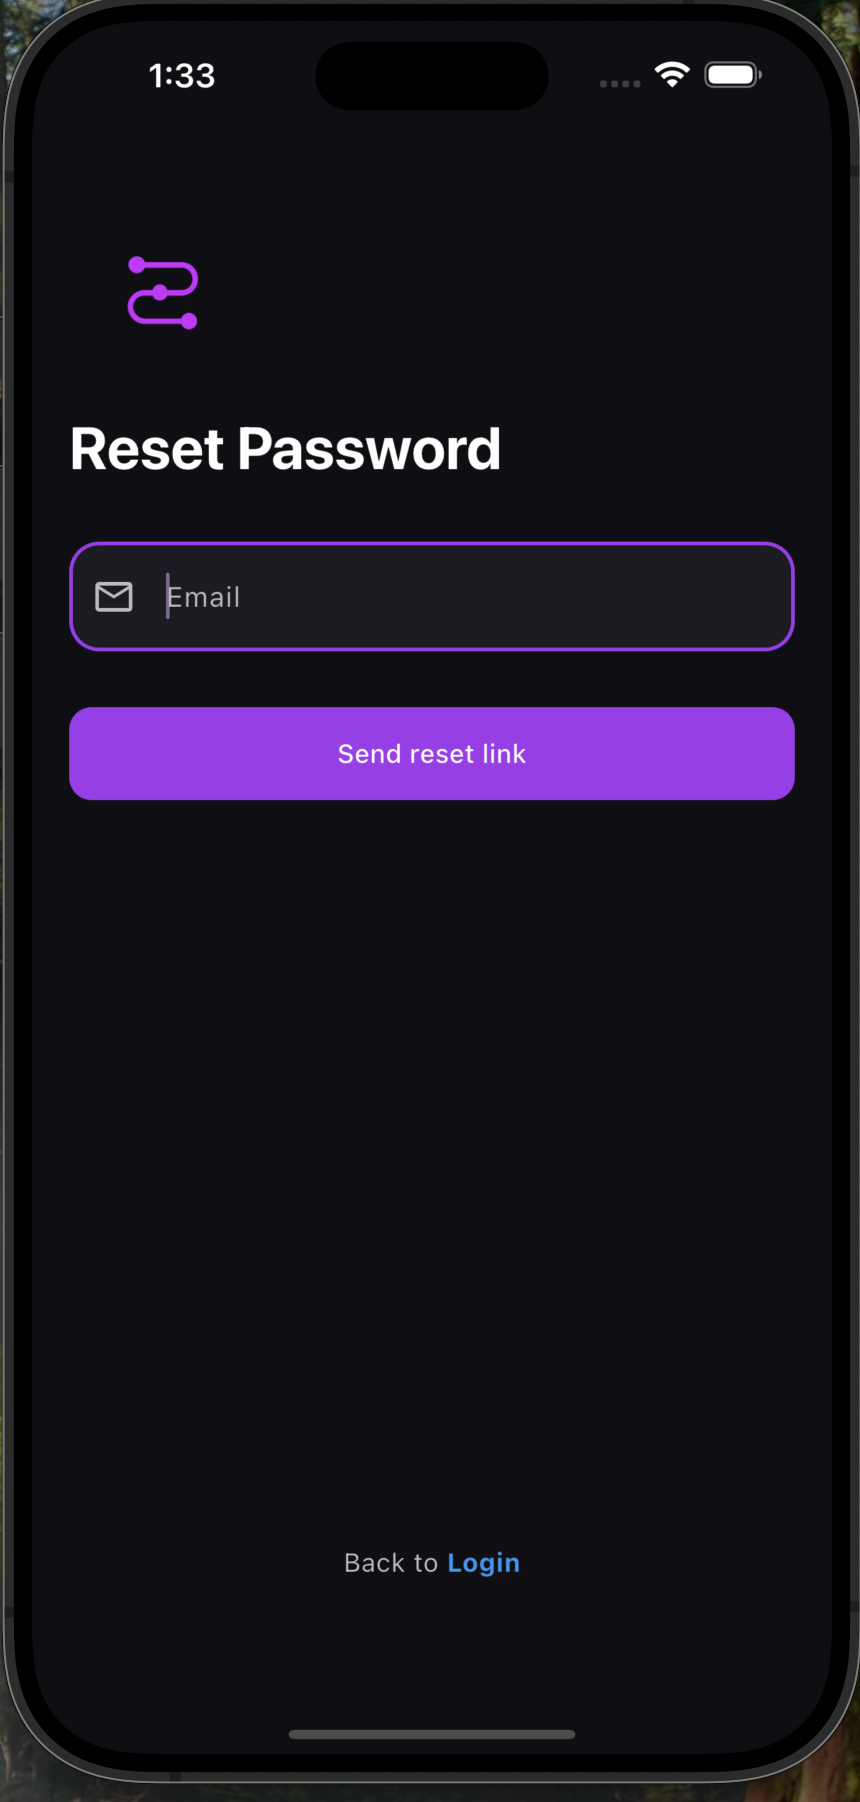
\includegraphics[width=0.42\textwidth]{images/mobile-app/auth-pages/auth-reset-D.png}
    \caption{Password Recovery Screen}
    \label{fig:mobile-reset-password}
\end{figure}

\vspace{0.2cm}
\noindent\textbf{Behavior \& Logical Flows}

\begin{itemize}
    \item Requests the user's registered email address.
    \item Sends a password reset request through the backend API.
    \item Displays loading indicators while waiting for server responses.
    \item Shows success or error messages according to the API response.
    \item Redirects users to create a new password after successful verification.
\end{itemize}

%%%%%%%%%%%%%%%%%%%%%%%%%%%%%%%%%%%%%%%%%%%%%%%%%%%%%%%%%%%%

\subsubsection{Reset Password Screen}

\begin{figure}[H]
    \centering
    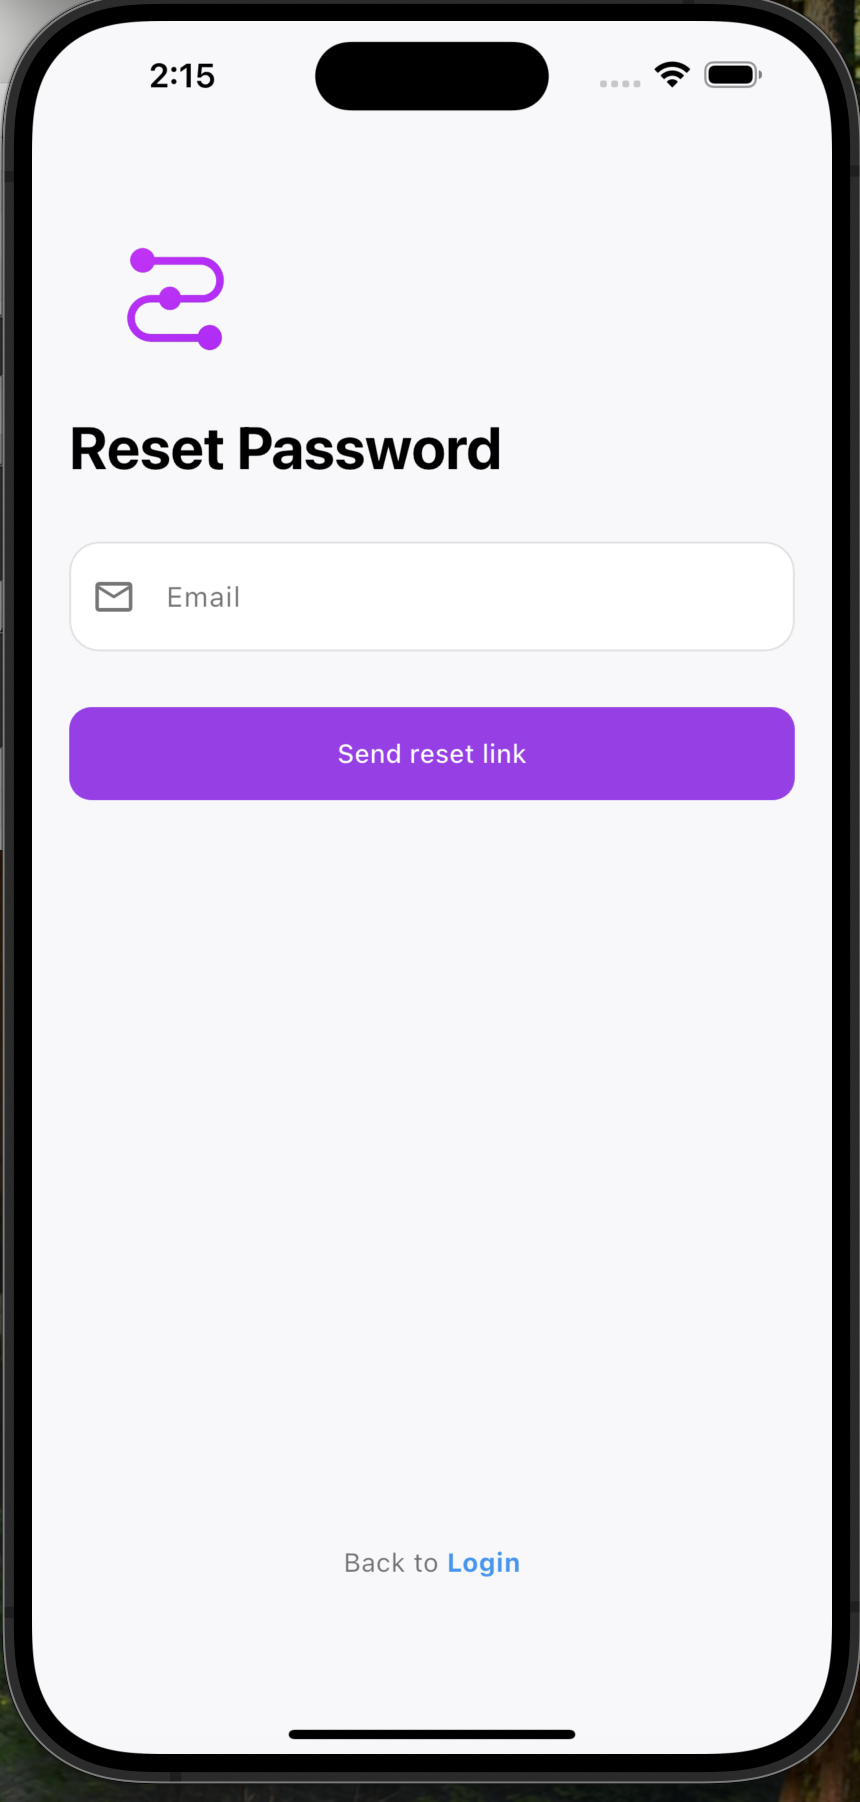
\includegraphics[width=0.42\textwidth]{images/mobile-app/auth-pages/auth-reset-L.png}
    \caption{Reset Password Screen}
    \label{fig:mobile-new-password}
\end{figure}

\vspace{0.2cm}
\noindent\textbf{Behavior \& Logical Flows}

\begin{itemize}
    \item Allows users to enter and confirm a new password.
    \item Validates password strength and confirmation before submission.
    \item Sends the updated password securely to the backend.
    \item Displays confirmation messages after a successful password update.
\end{itemize}

%%%%%%%%%%%%%%%%%%%%%%%%%%%%%%%%%%%%%%%%%%%%%%%%%%%%%%%%%%%%

\subsubsection{Authentication Flow}

\vspace{0.2cm}
\noindent\textbf{Behavior \& Logical Flows}

\begin{itemize}
    \item Users submit their authentication credentials through the mobile interface.
    \item The application validates all input fields locally before communicating with the backend.
    \item Authentication requests are transmitted securely using REST APIs.
    \item After successful authentication, the received JWT access token is stored locally using SharedPreferences.
    \item The stored token is automatically attached to subsequent API requests, enabling secure access to protected resources without requiring repeated logins.
\end{itemize}